\documentclass[11pt]{article}

\usepackage[letterpaper,margin=1in]{geometry}
\usepackage{amsmath,amssymb}
\usepackage{tikz}
\usepackage{enumitem}
\usepackage{fancyhdr}
\usepackage[most]{tcolorbox}
\usepackage{array}
\usepackage{titlesec}
\usepackage{xcolor}

\definecolor{fangblue}{RGB}{20,60,110}
\definecolor{fanggray}{RGB}{90,90,90}
\definecolor{boxgray}{RGB}{245,245,245}
\definecolor{reasonclr}{RGB}{70,100,150}   % step reasons
\definecolor{levE}{RGB}{20,120,60}          % Easy  (green)
\definecolor{levM}{RGB}{200,120,0}          % Medium (amber)
\definecolor{levH}{RGB}{190,40,40}          % Hard  (red)

\pagestyle{fancy}
\fancyhf{}
\renewcommand{\headrulewidth}{0.4pt}
\renewcommand{\footrulewidth}{0.4pt}
\lhead{\small\itshape Algebra \& Geometry Practice}
\rhead{\small\itshape FangMath}
\lfoot{\small\textcopyright\ 2026 FangMath $\cdot$ All rights reserved.}
\rfoot{\small\thepage}

\titleformat{\section}{\large\bfseries\color{fangblue}}{\thesection.}{0.6em}{}
\titleformat{\subsection}{\normalsize\bfseries}{}{0em}{}
\setlength{\parindent}{0pt}
\setlength{\parskip}{4pt}

\newtcolorbox{keybox}{colback=boxgray,colframe=fangblue,boxrule=0.6pt,
  arc=2pt,left=8pt,right=8pt,top=6pt,bottom=6pt}

\newcommand{\model}[1]{\textit{Model.}\ \ #1\par\vspace{4pt}}

% ruled writing lines for student work: \lines{n} draws n blank lines
\newcommand{\lines}[1]{\par\nobreak\vspace{2mm}%
  \foreach \x in {1,...,#1}{\noindent\textcolor{gray!55}{\rule{\linewidth}{0.3pt}}\par\vspace{0.8cm}}}

\begin{document}

\begin{center}
  {\LARGE\bfseries\color{fangblue} Algebra \& Geometry Practice Packet}\\[6pt]
  {\color{fanggray} Solving Equations $\cdot$ Quadratics $\cdot$ Radical Functions $\cdot$ Geometry}
\end{center}

\vspace{4pt}
\begin{center}
\begin{tabular}{@{}p{7.5cm}@{\hspace{1cm}}p{5cm}@{}}
\textbf{Name:} \underline{\hspace{5cm}} & \textbf{Date:} \underline{\hspace{3.5cm}}
\end{tabular}
\end{center}

\vspace{4pt}\hrule\vspace{8pt}

This packet has three difficulty levels throughout: \textbf{Easy}, \textbf{Medium},
and \textbf{Hard}. Each topic opens with a worked \emph{Model}, followed by similar practice.
Full solutions are in the Answer Key at the end.

% =====================================================================
\section{Solving Linear Equations}

\subsection*{\textcolor{levE}{Easy} --- One-Step Equations}
\textit{Model.}\ \ Solve $x + 7 = 12$.
\begin{align*}
x + 7 &= 12 &&\color{reasonclr}\text{original equation}\\
x &= 12 - 7 &&\color{reasonclr}\text{subtract 7 from both sides}\\
x &= 5 &&\color{reasonclr}\text{simplify}
\end{align*}
Solve each: \quad
(a) $x - 4 = 9$ \quad (b) $5x = 35$ \quad (c) $\dfrac{x}{3} = 6$ \quad (d) $x + 12 = 20$
\lines{4}

\subsection*{\textcolor{levM}{Medium} --- Two-Step Equations}
\textit{Model.}\ \ Solve $2x + 3 = 11$.
\begin{align*}
2x + 3 &= 11 &&\color{reasonclr}\text{original equation}\\
2x &= 8 &&\color{reasonclr}\text{subtract 3 from both sides}\\
x &= 4 &&\color{reasonclr}\text{divide both sides by 2}
\end{align*}
Solve each: \quad
(a) $3x - 5 = 16$ \quad (b) $4x + 7 = 31$ \quad (c) $\dfrac{x}{2} - 3 = 5$ \quad (d) $-2x + 9 = 1$
\lines{4}

\subsection*{\textcolor{levH}{Hard} --- Multi-Step Equations}
\textit{Model.}\ \ Solve $3(x-2) + 4 = 2x + 5$.
\begin{align*}
3(x-2) + 4 &= 2x + 5 &&\color{reasonclr}\text{original equation}\\
3x - 6 + 4 &= 2x + 5 &&\color{reasonclr}\text{distribute the 3}\\
3x - 2 &= 2x + 5 &&\color{reasonclr}\text{combine like terms}\\
x - 2 &= 5 &&\color{reasonclr}\text{subtract } 2x \text{ from both sides}\\
x &= 7 &&\color{reasonclr}\text{add 2 to both sides}
\end{align*}
Solve each:
\begin{enumerate}[label=(\alph*),leftmargin=2em,itemsep=6pt]
\item $2(x + 3) = x + 10$ \lines{2}
\item $5x - 2 = 3x + 8$ \lines{2}
\item $4(x - 1) + 2 = 2(x + 3)$ \lines{2}
\item $3x + 2(x - 1) = 18$ \lines{2}
\end{enumerate}
\vspace{2mm}

% =====================================================================
\section{Solving Quadratics by Factoring (Zero-Product Property)}

\begin{keybox}
\textbf{Zero-Product Property.} If $A \cdot B = 0$, then $A = 0$ \emph{or} $B = 0$.
So a quadratic in factored form is solved by setting each factor equal to $0$.
\end{keybox}

\subsection*{\textcolor{levE}{Easy} --- Already Factored}
\textit{Model.}\ \ Solve $(x+1)(x-2) = 0$.
\begin{align*}
(x+1)(x-2) &= 0 &&\color{reasonclr}\text{original equation}\\
x+1 = 0 \ \ &\text{or} \ \ x-2 = 0 &&\color{reasonclr}\text{zero-product property}\\
x = -1 \ \ &\text{or} \ \ x = 2 &&\color{reasonclr}\text{solve each factor}
\end{align*}
Solve each: \quad
(a) $(x-3)(x+5) = 0$ \quad (b) $(x+4)(x-6) = 0$ \quad (c) $x(x-7) = 0$ \quad (d) $(2x-1)(x+3) = 0$
\lines{4}

\subsection*{\textcolor{levM}{Medium} --- Factor First (leading coefficient $= 1$)}
\textit{Model.}\ \ Solve $x^2 + 5x + 6 = 0$.
\begin{align*}
x^2 + 5x + 6 &= 0 &&\color{reasonclr}\text{original equation}\\
(x+2)(x+3) &= 0 &&\color{reasonclr}\text{factor: } 2\cdot 3 = 6,\ 2+3 = 5\\
x+2 = 0 \ \ &\text{or} \ \ x+3 = 0 &&\color{reasonclr}\text{zero-product property}\\
x = -2 \ \ &\text{or} \ \ x = -3 &&\color{reasonclr}\text{solve each factor}
\end{align*}
Solve each: \quad
(a) $x^2 + 7x + 12 = 0$ \quad (b) $x^2 - 5x + 6 = 0$ \quad (c) $x^2 - x - 12 = 0$ \quad
(d) $x^2 + 2x - 15 = 0$
\lines{5}

\subsection*{\textcolor{levH}{Hard} --- Factor First (leading coefficient $\neq 1$)}
\textit{Model.}\ \ Solve $2x^2 + 7x + 3 = 0$.
\begin{align*}
2x^2 + 7x + 3 &= 0 &&\color{reasonclr}\text{original equation}\\
(2x+1)(x+3) &= 0 &&\color{reasonclr}\text{factor (product } 6,\ \text{sum } 7)\\
2x+1 = 0 \ \ &\text{or} \ \ x+3 = 0 &&\color{reasonclr}\text{zero-product property}\\
x = -\tfrac12 \ \ &\text{or} \ \ x = -3 &&\color{reasonclr}\text{solve each factor}
\end{align*}
Solve each: \quad
(a) $3x^2 - 10x + 8 = 0$ \quad (b) $2x^2 - 5x - 3 = 0$ \quad (c) $6x^2 + x - 2 = 0$ \quad
(d) $4x^2 - 4x - 3 = 0$
\lines{5}

% =====================================================================
\section{Solving Quadratics by the Quadratic Formula}

\begin{keybox}
\textbf{Quadratic Formula.} For $ax^2 + bx + c = 0$ \ ($a \neq 0$):
\[
x = \frac{-b \pm \sqrt{b^2 - 4ac}}{2a}.
\]
The value under the root, $b^2 - 4ac$, is the \emph{discriminant}: positive $\Rightarrow$ two
solutions, zero $\Rightarrow$ one, negative $\Rightarrow$ no real solution.
\end{keybox}

\textit{Model.}\ \ Solve $x^2 - 5x + 6 = 0$ \ ($a=1,\ b=-5,\ c=6$).
\begin{align*}
x &= \frac{-b \pm \sqrt{b^2 - 4ac}}{2a} &&\color{reasonclr}\text{quadratic formula}\\[2pt]
x &= \frac{-(-5) \pm \sqrt{(-5)^2 - 4(1)(6)}}{2(1)} &&\color{reasonclr}\text{substitute } a,\,b,\,c\\[2pt]
x &= \frac{5 \pm \sqrt{25 - 24}}{2} = \frac{5 \pm 1}{2} &&\color{reasonclr}\text{simplify under the root}\\[2pt]
x &= 3 \quad\text{or}\quad x = 2 &&\color{reasonclr}\text{the two solutions}
\end{align*}

Solve each with the quadratic formula:
\begin{enumerate}[label=(\alph*),leftmargin=2em,itemsep=6pt]
\item $x^2 + 3x - 10 = 0$ \lines{3}
\item $x^2 - 2x - 8 = 0$ \lines{3}
\item $2x^2 + 5x - 3 = 0$ \lines{3}
\item $x^2 - 4x + 1 = 0$ \quad \emph{(leaves a radical)} \lines{3}
\end{enumerate}
\vspace{2mm}

% =====================================================================
\section{Radical Functions: Domain \& Range}

\subsection*{Square-Root Functions}
\begin{keybox}
For a square root $y = \sqrt{\text{(radicand)}}$, the radicand must be $\ge 0$
(you cannot take the square root of a negative). Solve radicand $\ge 0$ to get the domain;
the output of a square root is always $\ge 0$.
\end{keybox}

\textit{Model.}\ \ Find the domain and range of $y = \sqrt{x+1}$.
\begin{align*}
x + 1 &\ge 0 &&\color{reasonclr}\text{the radicand cannot be negative}\\
x &\ge -1 &&\color{reasonclr}\text{subtract 1 from both sides}
\end{align*}
Domain: $x \ge -1,\ [-1,\infty)$. \quad Range: $y \ge 0,\ [0,\infty)$ \ (a square root is never negative).

\begin{center}
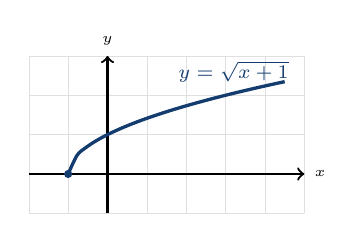
\begin{tikzpicture}[scale=0.5]
  \draw[step=1,gray!25,very thin] (-2,-1) grid (5,3);
  \draw[->,thick] (-2,0)--(5,0) node[right]{\tiny $x$};
  \draw[->,thick] (0,-1)--(0,3) node[above]{\tiny $y$};
  \draw[domain=-1:4.5,smooth,variable=\x,fangblue,very thick] plot ({\x},{sqrt(\x+1)});
  \filldraw[fangblue] (-1,0) circle (2.5pt);
  \node[fangblue] at (3.2,2.6) {\scriptsize $y=\sqrt{x+1}$};
\end{tikzpicture}
\end{center}

State the domain and range: \quad
(a) $y = \sqrt{x-3}$ \quad (b) $y = \sqrt{x+5}$ \quad (c) $y = \sqrt{2x-4}$ \quad (d) $y = \sqrt{x}+2$
\lines{4}

\subsection*{Cube-Root Functions}
\begin{keybox}
A cube root $y = \sqrt[3]{\text{(radicand)}}$ accepts \textbf{every} real number (negatives are
fine, since $\sqrt[3]{-8} = -2$). So both the domain and range are all real numbers.
\end{keybox}

\textit{Model.}\ \ Find the domain and range of $y = \sqrt[3]{x-1}$.
\begin{align*}
x - 1 &: \ \text{no restriction} &&\color{reasonclr}\text{a cube root is defined for every real number}\\
&&&(\text{e.g. } \sqrt[3]{-8} = -2)
\end{align*}
Domain: all reals $(-\infty,\infty)$. \quad Range: all reals $(-\infty,\infty)$.

\begin{center}
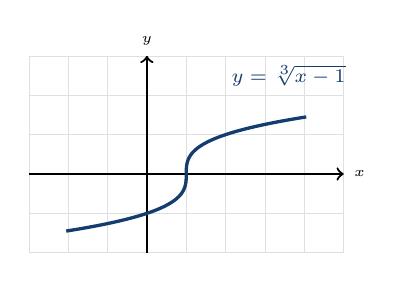
\begin{tikzpicture}[scale=0.5]
  \draw[step=1,gray!25,very thin] (-3,-2) grid (5,3);
  \draw[->,thick] (-3,0)--(5,0) node[right]{\tiny $x$};
  \draw[->,thick] (0,-2)--(0,3) node[above]{\tiny $y$};
  % parametric: let y = t, then x = t^3 + 1 (avoids fractional powers of negatives)
  \draw[domain=-1.45:1.45,smooth,samples=60,variable=\t,fangblue,very thick]
        plot ({\t*\t*\t + 1},{\t});
  \node[fangblue] at (3.6,2.5) {\scriptsize $y=\sqrt[3]{x-1}$};
\end{tikzpicture}
\end{center}

State the domain and range: \quad
(a) $y = \sqrt[3]{x+4}$ \quad (b) $y = \sqrt[3]{x}-2$ \quad (c) $y = \sqrt[3]{2x-6}$ \quad
(d) $y = \sqrt[3]{x-1}+3$
\lines{4}

% =====================================================================
\section{Geometry}

\subsection*{Sum of Interior Angles of a Polygon}
\begin{keybox}
The interior angles of a polygon with $n$ sides add up to
\[
(n - 2)\cdot 180^\circ.
\]
\end{keybox}
\textit{Model.}\ \ Find the interior-angle sum of a pentagon ($n = 5$).
\begin{align*}
\text{sum} &= (n-2)\cdot 180^\circ &&\color{reasonclr}\text{polygon angle-sum formula}\\
&= (5-2)\cdot 180^\circ &&\color{reasonclr}\text{substitute } n = 5\\
&= 3 \cdot 180^\circ = 540^\circ &&\color{reasonclr}\text{simplify}
\end{align*}
Find the interior-angle sum: \quad
(a) hexagon ($n=6$) \quad (b) octagon ($n=8$) \quad (c) quadrilateral ($n=4$) \quad
(d) decagon ($n=10$)
\lines{3}

\subsection*{Classifying a Quadrilateral from Four Vertices}
\begin{keybox}
Plot the four points, then use the \textbf{distance formula} for side lengths and \textbf{slopes}
for direction:
\begin{itemize}[nosep,leftmargin=1.4em]
\item Both pairs of opposite sides parallel $\Rightarrow$ \textbf{parallelogram}.
\item Parallelogram $+$ all four sides equal $\Rightarrow$ \textbf{rhombus}.
\item Parallelogram $+$ right angles $\Rightarrow$ \textbf{rectangle}.
\item All four sides equal \emph{and} right angles $\Rightarrow$ \textbf{square}.
\end{itemize}
\end{keybox}
\textit{Model.}\ \ Classify $A(0,0),\,B(4,0),\,C(4,3),\,D(0,3)$.
\begin{align*}
AB = DC &= 4,\quad BC = AD = 3 &&\color{reasonclr}\text{side lengths (distance formula)}\\
AB \text{ horizontal},\ &BC \text{ vertical} &&\color{reasonclr}\text{so consecutive sides are perpendicular}\\
&\Rightarrow \textbf{rectangle} &&\color{reasonclr}\text{has right angles, but } 4 \neq 3 \text{ so not a square}
\end{align*}
Classify each quadrilateral $ABCD$:
\begin{enumerate}[label=(\alph*),leftmargin=2em,itemsep=6pt]
\item $A(0,0),\,B(3,0),\,C(3,3),\,D(0,3)$ \lines{2}
\item $A(0,0),\,B(5,0),\,C(5,2),\,D(0,2)$ \lines{2}
\item $A(3,0),\,B(0,2),\,C(-3,0),\,D(0,-2)$ \lines{2}
\item $A(0,0),\,B(4,0),\,C(6,3),\,D(2,3)$ \lines{2}
\end{enumerate}
\vspace{2mm}

\subsection*{Surface Area of a Cylinder}
\begin{keybox}
A cylinder with radius $r$ and height $h$ has surface area
\[
SA = 2\pi r^2 + 2\pi r h \qquad (\text{two circular ends} + \text{the side}).
\]
\end{keybox}
\textit{Model.}\ \ Find the surface area for $r = 3,\ h = 5$.
\begin{align*}
SA &= 2\pi r^2 + 2\pi r h &&\color{reasonclr}\text{surface-area formula}\\
&= 2\pi(3)^2 + 2\pi(3)(5) &&\color{reasonclr}\text{substitute } r = 3,\ h = 5\\
&= 18\pi + 30\pi &&\color{reasonclr}\text{simplify each term}\\
&= 48\pi \approx 150.8 &&\color{reasonclr}\text{combine (square units)}
\end{align*}
Find the surface area (leave in terms of $\pi$, then round to one decimal): \quad
(a) $r=2,\ h=6$ \quad (b) $r=5,\ h=10$ \quad (c) $r=4,\ h=7$ \quad (d) $r=1,\ h=8$
\lines{4}

% =====================================================================
\newpage
\section{Answer Key}

\subsection*{1. Solving Linear Equations}
\textbf{Easy:} (a) $x=13$ \quad (b) $x=7$ \quad (c) $x=18$ \quad (d) $x=8$. \\
\textbf{Medium:} (a) $x=7$ \quad (b) $x=6$ \quad (c) $x=16$ \quad (d) $x=4$. \\
\textbf{Hard:} (a) $2x+6=x+10 \Rightarrow x=4$ \quad (b) $2x=10 \Rightarrow x=5$ \quad
(c) $4x-2=2x+6 \Rightarrow x=4$ \quad (d) $5x-2=18 \Rightarrow x=4$.

\subsection*{2. Quadratics by Factoring}
\textbf{Easy:} (a) $x=3,\,-5$ \quad (b) $x=-4,\,6$ \quad (c) $x=0,\,7$ \quad (d) $x=\tfrac12,\,-3$. \\
\textbf{Medium:} (a) $(x+3)(x+4)\Rightarrow x=-3,-4$ \quad (b) $(x-2)(x-3)\Rightarrow x=2,3$ \quad
(c) $(x-4)(x+3)\Rightarrow x=4,-3$ \quad (d) $(x+5)(x-3)\Rightarrow x=-5,3$. \\
\textbf{Hard:} (a) $(3x-4)(x-2)\Rightarrow x=\tfrac43,2$ \quad (b) $(2x+1)(x-3)\Rightarrow x=-\tfrac12,3$ \quad
(c) $(3x+2)(2x-1)\Rightarrow x=-\tfrac23,\tfrac12$ \quad (d) $(2x-3)(2x+1)\Rightarrow x=\tfrac32,-\tfrac12$.

\subsection*{3. Quadratic Formula}
(a) $x=\dfrac{-3\pm\sqrt{49}}{2}=\dfrac{-3\pm7}{2}\Rightarrow x=2,-5$. \quad
(b) $x=\dfrac{2\pm\sqrt{36}}{2}=\dfrac{2\pm6}{2}\Rightarrow x=4,-2$. \\
(c) $x=\dfrac{-5\pm\sqrt{49}}{4}=\dfrac{-5\pm7}{4}\Rightarrow x=\tfrac12,-3$. \quad
(d) $x=\dfrac{4\pm\sqrt{12}}{2}=2\pm\sqrt3$ (about $3.73$ and $0.27$).

\subsection*{4. Radical Functions}
\textbf{Square root} (range is $y\ge 0$ for a--c): \\
(a) $x\ge 3,\ [3,\infty)$; \ $y\ge 0$. \quad (b) $x\ge -5,\ [-5,\infty)$; \ $y\ge 0$. \quad
(c) $2x-4\ge0\Rightarrow x\ge 2$; \ $y\ge 0$. \quad (d) $x\ge 0$; \ range $y\ge 2$ (the $+2$ lifts it). \\
\textbf{Cube root} (all reals for both, in every case): \\
(a)--(d) Domain: all reals $(-\infty,\infty)$; \ Range: all reals $(-\infty,\infty)$.

\subsection*{5. Geometry}
\textbf{Interior angles:} (a) $720^\circ$ \quad (b) $1080^\circ$ \quad (c) $360^\circ$ \quad (d) $1440^\circ$. \\
\textbf{Classify:} (a) all sides $=3$ with right angles $\Rightarrow$ \textbf{square}. \quad
(b) sides $5$ and $2$ with right angles $\Rightarrow$ \textbf{rectangle}. \\
(c) all sides $=\sqrt{13}$, no right angle $\Rightarrow$ \textbf{rhombus}. \quad
(d) opposite sides equal/parallel ($AB=DC=(4,0)$, $AD=BC=(2,3)$), not equal adjacent, no right angle $\Rightarrow$ \textbf{parallelogram}. \\
\textbf{Cylinder surface area:} (a) $32\pi\approx100.5$ \quad (b) $150\pi\approx471.2$ \quad
(c) $88\pi\approx276.5$ \quad (d) $18\pi\approx56.5$ square units.

\end{document}
